\documentclass{article}
\newcommand\numberthis{\addtocounter{equation}{1}\tag{\theequation}}
\usepackage{geometry}
\usepackage{bm}
\usepackage[colorlinks=true, urlcolor=blue, pdfborder={0 0 0}]{hyperref}
\usepackage[yyyymmdd]{datetime}
\usepackage[inline,shortlabels]{enumitem}
\usepackage{mathtools}
\usepackage[dvipsnames]{xcolor}
\usepackage[framemethod=TikZ]{mdframed}
\usepackage{amsfonts}
\usepackage{float}
\usepackage{subcaption}
\usepackage{amsthm}
\usepackage{multirow}
\usepackage{amsmath}
\newtheoremstyle{problemstyle}{3pt}{3pt}{\normalfont}{}{\bfseries}{\normalfont\bfseries:}{.5em}{}
\theoremstyle{problemstyle}
\newmdtheoremenv[
  linewidth=1pt,
  linecolor=RoyalBlue,
  backgroundcolor=RoyalBlue!10,
  roundcorner=5pt,
  innertopmargin=6pt,
  innerbottommargin=6pt,
  innerleftmargin=6pt,
  innerrightmargin=6pt,
  nobreak=true
]{problem}{Problema}

% Solution
\newenvironment{solution}{%
  \begin{mdframed}[linewidth=0.8pt,roundcorner=5pt]%
  \noindent\textbf{Soluci\'on.}%
}{%
\hfill $ \diamond $ 
  \end{mdframed}%
}

% Make header with name and date etc.
\usepackage{fancyhdr}
\chead{\large M\'etodos Numericos I}
\lhead{Pedro D. Llerenas\quad \\\href{mailto:pedro.llerenas@cimat.mx}{pedro.llerenas@cimat.mx}}
\rhead{\today\\Examen Parcial I}
\thispagestyle{fancy}

\usepackage[utf8]{inputenc}
\usepackage[T1]{fontenc}
\setlength{\parindent}{0pt} % Don't indent new paragraphs
\setlength{\headheight}{24pt} 

\newcommand{\Z}{\mathbb Z}
\newcommand{\Q}{\mathbb Q}
\newcommand{\R}{\mathbb R}
\newcommand{\C}{\mathbb C}
\newcommand{\N}{\mathbb N}
\newcommand{\abs}[1]{\lvert #1 \rvert}
\newcommand{\norm}[1]{\lVert #1 \rVert}
\newcommand{\pde}[2]{\frac{\partial #1}{\partial #2}}
\newcommand{\bV}[1]{\mathbf{#1}}
\newcommand{\bmV}[1]{\mb{#1}}

% =======================================================================================%

\begin{document}
%begin problem 1
\begin{problem}
\textbf{(1 punto)}\\
Muestra te\'oricamente que la fuci\'on $ f(x) = e^x -\frac{4}{2+x} $ tiene una
ra\'iz en el intervalo $ [0,1] $. Aplica alguno de los algoritmos vistos en
clase para encontrar la ra\'iz de $ f(x) = 0 $. Explica los pasos que
realizaste para alcanzar la ra\'iz.
\end{problem}
%end problem 1

%begin solution 1
\begin{solution}
	Para demostrar que una funci\'on continua $ f:\R\to \R $ tiene una ra\'iz en
	un intervalo $ [a,b]\subset \R $, podemos utilizar el \textbf{teorema de
		Bolzano}, que nos asegura la existencia de \textbf{al menos} una ra\'iz $ c
		\in (a,b) $ si se cumple alguna de las siguientes dos condiciones:
	\begin{align*}
		f(a) < 0 < f(b)\qquad \text{\'o}\qquad f(a) > 0 > f(b).
	\end{align*}
	Es decir, que nuestra funci\'on tenga signo distinto en los puntos l\'imite
	del intervalo. Entonces, para aplicarlo a este ejercicio, primero notemos que
	\begin{align*}
		f(0) & = e^{0} - \frac{4}{2 + 0} \\
		     & = 1 - 2                   \\
		     & = -1.
	\end{align*}
	Mientras que
	\begin{align*}
		f(1) & = e^{1} - \frac{4}{2 + 1}    \\
		     & = e - \frac{4}{3}            \\
		     & > 0. \numberthis\label{eq:1}
	\end{align*}
	N\'otese que (\ref{eq:1}) se sigue de que $ e \approx 2.7 > 1.33... $. Entonces, como
	\begin{align*}
		f(0) < 0 < f(1),
	\end{align*}
	podemos concluir, por el teorema de Bolzano, que $ f $ tiene al menos una
	ra\'iz en el intervalo $ (0,1) $. Por completitud del ejercicio, tambi\'en
	mencionamos que claramente $ f $ no tiene ra\'ices en los puntos l\'imite.

	Ahora que hemos confirmado la existencia de al menos una ra\'iz, podemos
	aplicar un m\'etodo iterativo para encontrar una ra\'iz. Elegimos el
	\textbf{m\'etodo de bisecci\'on}. Decidimos usar este m\'etodo ya que es el
	m\'as simple y no requiere de pasos adicionales (como calcular derivadas o
	encontrar pseudo-inversas). El c\'odigo se encuentra en el archivo
	\texttt{p1.c}. Para compilar y ejecutar, usamos un \texttt{makefile}, que
	corremos usando el siguiente comando:
	\begin{center}
		\texttt{make run-p1 ARGS="1e-15 10000"}.
	\end{center}
	El primer argumento corresponde a la \textit{tolerancia}, y el segundo
	argumento corresponde al m\'aximo n\'umero de iteraciones. Al correr el
	programa, se imprime a la consola el siguiente mensaje:
	\begin{center}
		\texttt{Bisection method converged at iteration 49\\
			root = 0.478600339499129\\
			f(0.478600339499129) = -0.000000000000001}
	\end{center}
	Esto nos confirma que una ra\'iz que se encuentra en el intervalo $ (0,1) $ es
	\begin{align*}
		c = 0.478600339499129.
	\end{align*}
	Para llegar a este resultado, el algoritmo de bisecci\'on realiz\'o 49
	iteraciones. En cada iteraci\'on, busca el punto medio del intervalo dado, y
	eval\'ua la funci\'on en ese punto. Si es menor a la tolerancia, acabamos.
	Si no, reducimos el intervalo de b\'usqueda dependiendo del signo de la
	funci\'on en el punto medio y puntos extremos, buscando que el signo sea
	distinto.
\end{solution}
%end solution 1

% =======================================================================================%

%begin problem 2
\begin{problem}
\textbf{(2 puntos)}\\
Escribe un programa que calcule $ x(\sqrt{x+1}-\sqrt{x}) $ para $ x = 10^n $, con $ n = 1, 2, \dots, 20 $.
\begin{itemize}
	\item Grafica los resultados. Proporciona una explicaci\'on de los sucedido. \textbf{(1 punto)}
	\item Proporciona una expresi\'on alternativa y compara los resultados obtenidos. Explica. \textbf{(1 punto)}
\end{itemize}
\end{problem}
%end problem 2

%begin solution 2
\begin{solution}
  Para correr el programa, usar
  \begin{center}
    \texttt{make run-p2 ARGS="p2.txt p2\_new.txt"}
  \end{center}
  Esto nos genera 2 archivos, uno con la secuencia de la funci\'on sin modificar (p2.txt) y el otro contiene la secuencia con la funci\'on modificada.
	\begin{figure}[H]
		\begin{subfigure}{.45\textwidth}
			\centering
			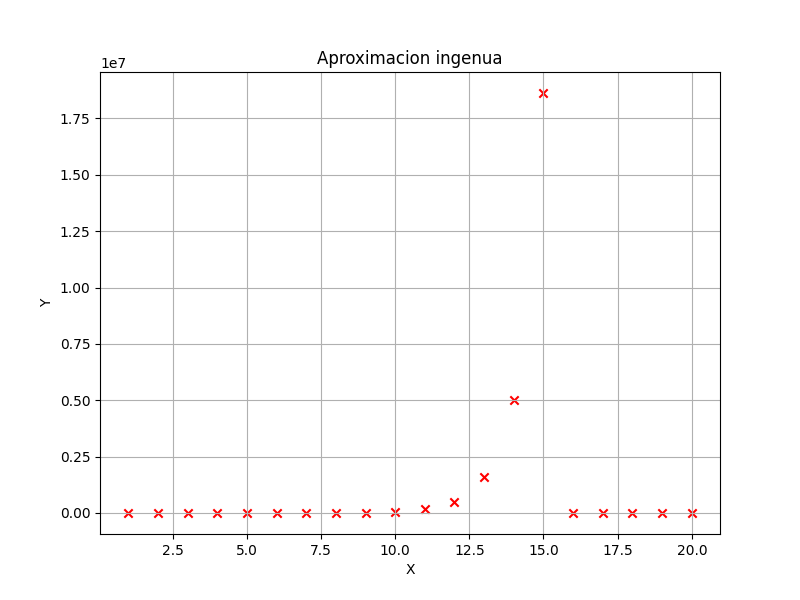
\includegraphics[width=0.95\textwidth]{p2_ing.png}
			\caption{$ x(\sqrt{x+1} - \sqrt{x}) $}
			\label{fig:f_ing}
		\end{subfigure}
		\hfill
		\begin{subfigure}{.45\textwidth}
			\centering
			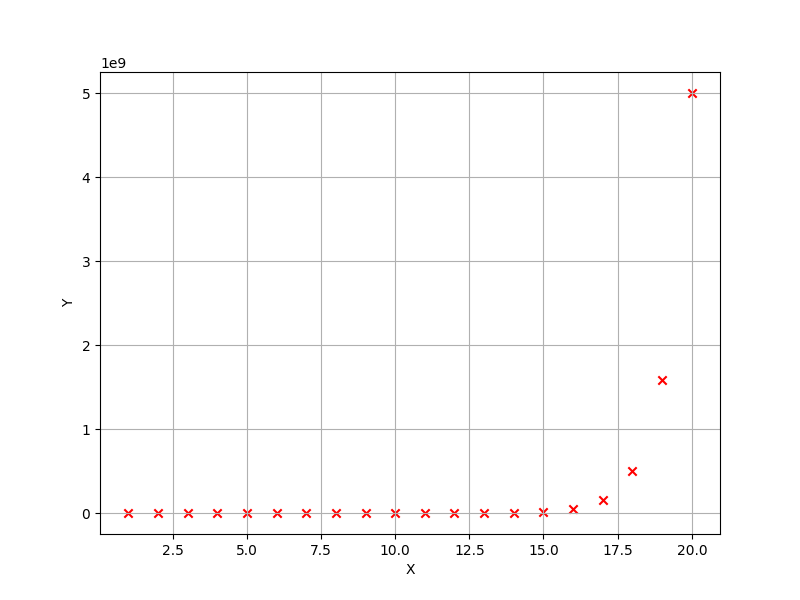
\includegraphics[width=0.95\textwidth]{p2.png}
			\caption{$\frac{x}{\sqrt{x+1} + \sqrt{x}}$}
			\label{fig:f_r}
		\end{subfigure}
		\caption{Comparaci\'on de gr\'aficas de la misma funci\'on, con diferente representaci\'on.}
	\end{figure}
	Notemos que al graficar los puntos de la funci\'on $ x(\sqrt{x+1} - \sqrt{x})
	$ (gr\'afica  \ref{fig:f_ing}), al principio de los valores de $ n $, no tenemos problemas. Sin embargo,
	cuando alcanzamos el valor $ n = 16 $, la expresi\'on resulta 0. Esto es
	debido a la precici\'on finita de punto flotante. Como $ \sqrt{x+1} $ y $
		\sqrt{x} $ son my similares para n\'umeros grandes, su diferencia es muy
	peque\~na en esos rangos, por lo que $ \sqrt{x+1} - \sqrt{x} = 0 $ para $
		x\geq 10^{16} $ de acuerdo a la precisi\'on de la m\'aquina.

	Para contrarestar esta limitante, evitamos el uso de la resta mediante manipulaci\'on algebr\'aica usando $ a^2-b^2 = (a+b)(a-b) $:
	\begin{align*}
		x(\sqrt{x + 1} - \sqrt{x}) & = x(\sqrt{x + 1} - \sqrt{x})\cdot \frac{\sqrt{x+1} + \sqrt{x}}{\sqrt{x+1}+\sqrt{x}} \\
		                           & = \frac{x(x+1-x)}{\sqrt{x+1}+\sqrt{x}}                                              \\
		                           & = \frac{x}{\sqrt{x+1}+\sqrt{x}}.
	\end{align*}
	Entonces, realizando nuevamente los c\'alculos, obtenemos la gr\'afica
	\ref{fig:f_r}, que muestra el comportamiento real esperado. Ahora, sin el t\'ermino que se vuelve 0 por el l\'imite de precisi\'on, la expresi\'on se evaul\'ua correctamente.
\end{solution}
%end solution 2

% =======================================================================================%

%begin problem 3
\begin{problem}
\textbf{(2 puntos)}\hfill

La ecuaci\'on $ f(x) = x - 3x^{-x} = 0 $ tiene una soluci\'on $ x^* \approx 1.05 $.
\begin{itemize}
	\item Analiza las siguientes iteraciones de punto fijo desde un punto de
	      vista te\'orico y determina si convergen hacia $ x^* $, adem\'as,
	      identifique cu\'al de los m\'etodos presenta una convergencia m\'as
	      r\'apida. \textbf{(1.5 puntos)}
	      \begin{center}
		      \begin{enumerate*}[label=(\roman*),itemjoin=\qquad]
			      \item $\displaystyle x_{n+1} = 3e^{-x_n} $,
			      \item $\displaystyle x_{n+1} = (2x_n + 3e^{-x_n})/3$,
			      \item $\displaystyle x_{n+1} = 1.05x_n + 3e^{-x_n} $,
			      \item $\displaystyle x_{n+1} = (x_n+3e^{-x_n})/2$
		      \end{enumerate*}
	      \end{center}

	\item Presenta una tabla de datos comparativos de tal manera que se alcance un error absoluto de al menos $ 10^{-10} $ considerando $ x_0 = 1.05 $. (\textbf{0.5 puntos})
\end{itemize}
\end{problem}
%end problem 3

%begin solution 3
\begin{solution}
Este programa se ejecuta usando
\begin{center}
  \texttt{make run-p3}.
\end{center}
Nos genera 4 archivos:
\begin{center}
		\texttt{p3\_1.txt} --- Tabla de iteraciones de $ g_1 $.\\
		\texttt{p3\_2.txt} --- Tabla de iteraciones de $ g_2 $.\\
    \texttt{p3\_3.txt} --- Tabla de iteraciones de $ g_3 $.\\
    \texttt{p3\_4.txt} --- Tabla de iteraciones de $ g_4 $.
\end{center}

\begin{enumerate}
	\item $\displaystyle x_{n+1} = 3e^{-x_n} $,
	      Esta funci\'on no satisface la condici\'on de $ \abs{g'(x)} \leq k< 1 $. Efectivamente,
	      \begin{align*}
		      \abs{g_1'(x)} = 3e^{-x} > 1 \quad \forall x \leq 1.05
	      \end{align*}
	      Entonces, el teorema de punto fijo no nos garantiza la convergencia, ya que en ninguna vecindad del punto $ x=1.05 $ se logra cumplir esta propiedad.
	\item $\displaystyle x_{n+1} = (2x_n + 3e^{-x_n})/3$,
	      Para esta funci\'on, tenemos
	      \begin{align*}
		      \abs{g_2'(x)} =\frac{\abs{2 - 3e^{x}}}{3} < 1\qquad \forall x\in (1, 1.1)
	      \end{align*}
	      y tambi\'en $ g_2(x) \in (1,1.1) $ para $ x\in (1, 1.1) $. Es decir,
	      podemos aplicar el teorema de punto fijo con esperanza de obtener la
	      ra\'iz de $ f $.
	\item $\displaystyle x_{n+1} = 1.05x_n + 3e^{-x_n} $,
	      Esta funci\'on no tiene sentido ni considerarla, ya que
	      \begin{align*}
		      g_3(x) > x \qquad \forall x
	      \end{align*}
	      Es decir, no es posible que exista un punto fijo.
	\item $\displaystyle x_{n+1} = (x_n+3e^{-x_n})/2$
	      Para esta funci\'on verificamos que las condiciones se cumplen:
	      \begin{align*}
		      g_4(x) \in (1, 1.1) \qquad \forall x\in(1,1.1)
	      \end{align*}
	      y
	      \begin{align*}
		      \abs{g_4(x)} =\frac{\abs{1-3e^{-x}}}{2} < 1\qquad \forall x\in(1, 1.1)
	      \end{align*}
\end{enumerate}
Entonces, podemos concluir que, te\'oricamente, solo las opciones 3 y 4 convergen. Ahora bien, si queremos conocer cu\'al converge m\'as r\'apido, basta ver que
\begin{align*}
	\abs{g'_4(x)} = \frac{\abs{1-3e^{-x}}}{2} \leq \frac{\abs{2 - 3e^{x}}}{3}= \abs{g'_2(x)}.
\end{align*}
para $ x\in (1,1.1) $. Es decir, la constante de convergencia de $ g_4 $ es menor que la de $ g_2 $.

\begin{table}[H]
	\centering
	\begin{tabular}[H]{c|c|c|c|c}
		\hline
		n  & $ \abs{x_n - g_1(x_n)} $ & $ \abs{x_n - g_2(x_n)} $ & $ \abs{x_n - g_3(x_n)} $ & $ \abs{x_n - g_4(x_n)} $ \\
		\hline
		0  & 1.868$\times10^{-4}$     & 6.225$\times10^{-5}$     & 1.102$\times10^{0}$      & $9.33763\times10^{-15}$
		\\
		1  & 1.868$\times10^{-4}$     & 6.225$\times10^{-5}$     & 1.102$\times10^{0}$      & $9.33763\times10^{-05}$
		\\
		2  & 1.961$\times10^{-4}$     & 1.972$\times10^{-5}$     & 4.563$\times10^{-1}$     & $2.32798\times10^{-06}$
		\\
		3  & 2.059$\times10^{-4}$     & 6.244$\times10^{-6}$     & 3.513$\times10^{-1}$     & $5.80947\times10^{-08}$
		\\
		4  & 2.161$\times10^{-4}$     & 1.978$\times10^{-6}$     & 3.035$\times10^{-1}$     & $1.44972\times10^{-09}$
		\\
		5  & 2.269$\times10^{-4}$     & 6.263$\times10^{-7}$     & 2.779$\times10^{-1}$     & $3.61771\times10^{-11}$
		\\
		6  & 2.382$\times10^{-4}$     & 1.983$\times10^{-7}$     & 2.640$\times10^{-1}$     & $9.02611\times10^{-13}$
		\\
		7  & 2.501$\times10^{-4}$     & 6.281$\times10^{-8}$     & 2.570$\times10^{-1}$     & $2.24265\times10^{-14}$
		\\
		8  & 2.626$\times10^{-4}$     & 1.989$\times10^{-8}$     & 2.547$\times10^{-1}$     & $6.66134\times10^{-16}$  \\
		9  & 3.757$\times10^{-4}$     & 6.300$\times10^{-9}$     & 2.559$\times10^{-1}$     & ---                      \\
		10 & 2.895$\times10^{-4}$     & 1.995$\times10^{-9}$     & 2.596$\times10^{-1}$     & ---                      \\
		11 & 3.039$\times10^{-4}$     & 6.318$\times10^{-10}$    & 2.655$\times10^{-1}$     & ---                      \\
	\end{tabular}
	\caption{}\label{tab:}
\end{table}

\end{solution}
%end solution 3

% =======================================================================================%

%begin problem 4
\begin{problem}
\textbf{(5 puntos)}\hfill
Se requiere resolver un problema de difusi\'on del cual se obtiene un sistema de ecuaciones pentadiagonal. El sistema de ecuaciones tiene la siguiente forma
\begin{align*}
	\bV{Ax} = \bV{b},
\end{align*}
con
\begin{align*}
	-5x_{i-2} - 10x_{i-1} + 50x_{i} - 10x_{i+1} - 5x_{i+1} = 200,\qquad i = 3,\dots,1998.
\end{align*}
En los extremos de la matriz $ \bV{A} $ se eliminan los t\'erminos que quedan fuera (cuando el \'indice es negativo o mayor a 2000). As\'i,
\begin{itemize}
	\item La primera ecuaci\'on es: $ 50x_1 - 10x_2 - 5x_3 = 40 $;
	\item La segunda ecuaci\'on es: $ -10x_1 + 50x_2 - 10x_3 - 5x_4 = 100 $;
	\item La pen\'ultima ecuaci\'on es: $ -5x_{1997} - 10x_{1998} + 50x_{1999} - 10x_{2000} = 100 $;
	\item La \'ultima ecuaci\'on es: $ -5x_1 - 10x_{1999} - 50x_{2000} = 40 $.
\end{itemize}
Con el sistema generado (\textbf{1 punto}), obtener:
\begin{itemize}
	\item La soluci\'on del sistema de ecauciones con dos m\'etodos distintos.
	      Decir por qu\'e utilizaste esos m\'etodos de soluci\'on. (\textbf{2
		      puntos})
	\item Los eigenvectores correspondientes a la matriz $ \bV{A} $. Presentar
	      los 10 eigenvalores m\'as peque\~nos y los 10 m\'as grandes. (\textbf{2
		      puntos})
\end{itemize}
\end{problem}
%end problem 3

%begin solution 3
\begin{solution}

	Compilamos y ejecutamos con
	\begin{center}
		\texttt{make run-p4}
	\end{center}
	Guardamos los el vector de constantes como \texttt{vector.txt}, y la matriz de $ 2000\times 2000 $ como \texttt{matrix.txt}.

	Para resolver el sistema, usamos el m\'etodo de gradiente conjugado y el
	m\'etodo de Gauss-Siedel. Elegimos estos ya que la matriz es diagonalmente
	dominante, simetrica y positiva definida. Espec\'ificamente, estos m\'etodos
	(en teor\'ia) trabajan mejor con matrices con muchos ceros, a comparaci\'on
	de otras como LU o por medio de factorizaci\'on de Cholesky.

	Con la ejecuci\'on mencionada anteriormente, obtenemos 2 archivos:
	\begin{center}
		\texttt{conjugate\_s.txt} y \texttt{gauss\_s.txt}.
	\end{center}
	El m\'etodo de gradiente conjugado converge\footnote{como el vector inicial se genera aleatoriamente, puede que la convergencia sea distinta} en 28 iteraciones con una tolerancia de $ 10^{-12} $, mientras que el de Gauss-Siedel en 40, con la misma tolerancia.

	Para encontrar los eigenvectores y eigenvalores, usamos el m\'etodo de la
	potencia y potencia inversa. En contraste, el m\'etodo de iteraci\'on de
	subespacio parece ser m\'as ineficiente debido al proceso de Jacobi
	intermedio que se utiliza para rotar la matriz (en este caso, gigantesca). Al ejecutar el programa, obtenemos 4 archivos.

	\begin{center}
		\texttt{biggest.txt} --- Eigenvalores m\'as grandes.\\
		\texttt{smallest.txt} --- Eigenvalores m\'as peque\~nos.\\
		\texttt{biggest\_evec.txt} --- Eigenvectores correspondientes a los eigenvalores m\'as grandes.\\
		\texttt{smallest\_evec.txt} --- Eigenvectores correspondientes a los eigenvalores m\'as peque\~nos.
	\end{center}

	\begin{table}[H]
		\begin{center}
			\begin{tabular}{|c|c|c|}
				\hline
				n  & Grandes   & Peque\~nos \\
				\hline
				1  & 64.977933 & 20.001248  \\
				2  & 64.977284 & 20.012309  \\
				3  & 64.977484 & 20.012727  \\
				4  & 64.977752 & 20.012647  \\
				5  & 64.977983 & 20.012541  \\
				6  & 64.978182 & 20.012506  \\
				7  & 64.978342 & 20.012607  \\
				8  & 64.978473 & 20.013074  \\
				9  & 64.978581 & 20.014888  \\
				10 & 64.978674 & 20.019698  \\
				\hline
			\end{tabular}
		\end{center}
		\caption{Eigenvalores m\'as grandes y peque\~nos}
	\end{table}
  Notemos que no son estrictamente decrecientes/crecientes. Esto se debe a la
  imprecisi\'on de los puntos flotantes, y como una soluci\'on depende la otra
  (al hacer la reducci\'on), estos errores van acarreando. Estos resultados son con tolerancia de $ 10^{-5} $.
\end{solution}
%end solution 3

% =======================================================================================%
\end{document}
